%----------------------------------------------------------------------------------------
%	PACKAGES AND OTHER DOCUMENT CONFIGURATIONS
%----------------------------------------------------------------------------------------
\documentclass[a4paper,11pt]{article}
\usepackage[a4paper,textwidth=140mm,textheight=245mm]{geometry}
\usepackage[utf8]{inputenc}
\usepackage{listings}
\usepackage{graphicx}
\usepackage{mathtools}
\usepackage{subscript}
\usepackage{tikz}
\makeatletter
\renewcommand{\section}{\@startsection
   {section}%                         name
   {1}%                               level
   {0mm}%                             indent
   {-1.5\baselineskip}%               space above header
   {0.5\baselineskip}%                space under header
   {\sffamily\bfseries\upshape\normalsize}}% style
\renewcommand{\subsection}{\@startsection
   {subsection}%                      name
   {2}%                               level
   {0mm}%                             indent
   {-0.75\baselineskip}%              space above header
   {0.25\baselineskip}%               space under header
   {\rmfamily\normalfont\slshape\normalsize}}% style
\renewcommand{\subsubsection}{\@startsection
   {subsubsection}%                    name
   {3}%                               level
   {-10mm}%                             indent
   {-0.75\baselineskip}%              space above header
   {0.25\baselineskip}%               space under header
   {\rmfamily\normalfont\slshape\normalsize}}% style
\makeatother
\begin{document}

\begin{titlepage}
\title{TDDC93 Summary:}
\author{Martin Söderén\\ marso329@student.liu.se\\900929-1098}
\date{\today}
\maketitle
\vfill % Fill the rest of the page with whitespace
\thispagestyle{empty}
\end{titlepage}

%REQUIREMENTS
\section{Requirements}
are described in IEEE Standard 830 
\subsection{requirements analysis}
analyzing, documenting, validating and managing software or system requirements.
\subsection{consistent requirement}
The requirement does not contradict any other requirement and is fully consistent with all authoritative external documentation.
\subsection{Entity - Relationship}
mostly used to describe business processes. For example relations between managers in companies
\subsection{non-functional requirements}
 how a system will do something
\\bandwidth, availability,backup,documentation,maintainability
\subsection{functional requirements}
what a system will do
\\Authentication,Administrative functions,External Interfaces,Reporting Requirements,Historical Data
\subsection{UML}
% Graphic for TeX using PGF
% Title: /home/martin/Diagram1.dia
% Creator: Dia v0.97.2
% CreationDate: Sun Oct 26 15:45:36 2014
% For: martin
% \usepackage{tikz}
% The following commands are not supported in PSTricks at present
% We define them conditionally, so when they are implemented,
% this pgf file will use them.
\ifx\du\undefined
  \newlength{\du}
\fi
\setlength{\du}{15\unitlength}
\begin{tikzpicture}
\pgftransformxscale{1.000000}
\pgftransformyscale{-1.000000}
\definecolor{dialinecolor}{rgb}{0.000000, 0.000000, 0.000000}
\pgfsetstrokecolor{dialinecolor}
\definecolor{dialinecolor}{rgb}{1.000000, 1.000000, 1.000000}
\pgfsetfillcolor{dialinecolor}
\pgfsetlinewidth{0.100000\du}
\pgfsetdash{}{0pt}
\definecolor{dialinecolor}{rgb}{1.000000, 1.000000, 1.000000}
\pgfsetfillcolor{dialinecolor}
\fill (2.100000\du,6.600000\du)--(2.100000\du,8.000000\du)--(6.450000\du,8.000000\du)--(6.450000\du,6.600000\du)--cycle;
\definecolor{dialinecolor}{rgb}{0.000000, 0.000000, 0.000000}
\pgfsetstrokecolor{dialinecolor}
\draw (2.100000\du,6.600000\du)--(2.100000\du,8.000000\du)--(6.450000\du,8.000000\du)--(6.450000\du,6.600000\du)--cycle;
% setfont left to latex
\definecolor{dialinecolor}{rgb}{0.000000, 0.000000, 0.000000}
\pgfsetstrokecolor{dialinecolor}
\node at (4.275000\du,7.550000\du){Car};
\definecolor{dialinecolor}{rgb}{1.000000, 1.000000, 1.000000}
\pgfsetfillcolor{dialinecolor}
\fill (2.100000\du,8.000000\du)--(2.100000\du,8.400000\du)--(6.450000\du,8.400000\du)--(6.450000\du,8.000000\du)--cycle;
\definecolor{dialinecolor}{rgb}{0.000000, 0.000000, 0.000000}
\pgfsetstrokecolor{dialinecolor}
\draw (2.100000\du,8.000000\du)--(2.100000\du,8.400000\du)--(6.450000\du,8.400000\du)--(6.450000\du,8.000000\du)--cycle;
\definecolor{dialinecolor}{rgb}{1.000000, 1.000000, 1.000000}
\pgfsetfillcolor{dialinecolor}
\fill (2.100000\du,8.400000\du)--(2.100000\du,11.000000\du)--(6.450000\du,11.000000\du)--(6.450000\du,8.400000\du)--cycle;
\definecolor{dialinecolor}{rgb}{0.000000, 0.000000, 0.000000}
\pgfsetstrokecolor{dialinecolor}
\draw (2.100000\du,8.400000\du)--(2.100000\du,11.000000\du)--(6.450000\du,11.000000\du)--(6.450000\du,8.400000\du)--cycle;
% setfont left to latex
\definecolor{dialinecolor}{rgb}{0.000000, 0.000000, 0.000000}
\pgfsetstrokecolor{dialinecolor}
\node[anchor=west] at (2.250000\du,9.100000\du){+drive()};
% setfont left to latex
\definecolor{dialinecolor}{rgb}{0.000000, 0.000000, 0.000000}
\pgfsetstrokecolor{dialinecolor}
\node[anchor=west] at (2.250000\du,9.900000\du){+reverse()};
% setfont left to latex
\definecolor{dialinecolor}{rgb}{0.000000, 0.000000, 0.000000}
\pgfsetstrokecolor{dialinecolor}
\node[anchor=west] at (2.250000\du,10.700000\du){+open()};
\pgfsetlinewidth{0.100000\du}
\pgfsetdash{}{0pt}
\definecolor{dialinecolor}{rgb}{1.000000, 1.000000, 1.000000}
\pgfsetfillcolor{dialinecolor}
\fill (17.000000\du,6.550000\du)--(17.000000\du,7.950000\du)--(22.575000\du,7.950000\du)--(22.575000\du,6.550000\du)--cycle;
\definecolor{dialinecolor}{rgb}{0.000000, 0.000000, 0.000000}
\pgfsetstrokecolor{dialinecolor}
\draw (17.000000\du,6.550000\du)--(17.000000\du,7.950000\du)--(22.575000\du,7.950000\du)--(22.575000\du,6.550000\du)--cycle;
% setfont left to latex
\definecolor{dialinecolor}{rgb}{0.000000, 0.000000, 0.000000}
\pgfsetstrokecolor{dialinecolor}
\node at (19.787500\du,7.500000\du){MotorCycle};
\definecolor{dialinecolor}{rgb}{1.000000, 1.000000, 1.000000}
\pgfsetfillcolor{dialinecolor}
\fill (17.000000\du,7.950000\du)--(17.000000\du,8.350000\du)--(22.575000\du,8.350000\du)--(22.575000\du,7.950000\du)--cycle;
\definecolor{dialinecolor}{rgb}{0.000000, 0.000000, 0.000000}
\pgfsetstrokecolor{dialinecolor}
\draw (17.000000\du,7.950000\du)--(17.000000\du,8.350000\du)--(22.575000\du,8.350000\du)--(22.575000\du,7.950000\du)--cycle;
\definecolor{dialinecolor}{rgb}{1.000000, 1.000000, 1.000000}
\pgfsetfillcolor{dialinecolor}
\fill (17.000000\du,8.350000\du)--(17.000000\du,9.350000\du)--(22.575000\du,9.350000\du)--(22.575000\du,8.350000\du)--cycle;
\definecolor{dialinecolor}{rgb}{0.000000, 0.000000, 0.000000}
\pgfsetstrokecolor{dialinecolor}
\draw (17.000000\du,8.350000\du)--(17.000000\du,9.350000\du)--(22.575000\du,9.350000\du)--(22.575000\du,8.350000\du)--cycle;
% setfont left to latex
\definecolor{dialinecolor}{rgb}{0.000000, 0.000000, 0.000000}
\pgfsetstrokecolor{dialinecolor}
\node[anchor=west] at (17.150000\du,9.050000\du){+drive()};
\pgfsetlinewidth{0.100000\du}
\pgfsetdash{}{0pt}
\definecolor{dialinecolor}{rgb}{1.000000, 1.000000, 1.000000}
\pgfsetfillcolor{dialinecolor}
\fill (7.700000\du,6.500000\du)--(7.700000\du,7.900000\du)--(11.012500\du,7.900000\du)--(11.012500\du,6.500000\du)--cycle;
\definecolor{dialinecolor}{rgb}{0.000000, 0.000000, 0.000000}
\pgfsetstrokecolor{dialinecolor}
\draw (7.700000\du,6.500000\du)--(7.700000\du,7.900000\du)--(11.012500\du,7.900000\du)--(11.012500\du,6.500000\du)--cycle;
% setfont left to latex
\definecolor{dialinecolor}{rgb}{0.000000, 0.000000, 0.000000}
\pgfsetstrokecolor{dialinecolor}
\node at (9.356250\du,7.450000\du){Wheel};
\definecolor{dialinecolor}{rgb}{1.000000, 1.000000, 1.000000}
\pgfsetfillcolor{dialinecolor}
\fill (7.700000\du,7.900000\du)--(7.700000\du,8.300000\du)--(11.012500\du,8.300000\du)--(11.012500\du,7.900000\du)--cycle;
\definecolor{dialinecolor}{rgb}{0.000000, 0.000000, 0.000000}
\pgfsetstrokecolor{dialinecolor}
\draw (7.700000\du,7.900000\du)--(7.700000\du,8.300000\du)--(11.012500\du,8.300000\du)--(11.012500\du,7.900000\du)--cycle;
\definecolor{dialinecolor}{rgb}{1.000000, 1.000000, 1.000000}
\pgfsetfillcolor{dialinecolor}
\fill (7.700000\du,8.300000\du)--(7.700000\du,8.700000\du)--(11.012500\du,8.700000\du)--(11.012500\du,8.300000\du)--cycle;
\definecolor{dialinecolor}{rgb}{0.000000, 0.000000, 0.000000}
\pgfsetstrokecolor{dialinecolor}
\draw (7.700000\du,8.300000\du)--(7.700000\du,8.700000\du)--(11.012500\du,8.700000\du)--(11.012500\du,8.300000\du)--cycle;
\pgfsetlinewidth{0.100000\du}
\pgfsetdash{}{0pt}
\pgfsetdash{}{0pt}
\pgfsetbuttcap
{
\definecolor{dialinecolor}{rgb}{0.000000, 0.000000, 0.000000}
\pgfsetfillcolor{dialinecolor}
% was here!!!
\pgfsetarrowsend{to}
\definecolor{dialinecolor}{rgb}{0.000000, 0.000000, 0.000000}
\pgfsetstrokecolor{dialinecolor}
\draw (6.499287\du,8.274707\du)--(7.669116\du,7.998437\du);
}
\definecolor{dialinecolor}{rgb}{0.000000, 0.000000, 0.000000}
\pgfsetstrokecolor{dialinecolor}
\draw (6.848266\du,8.192291\du)--(7.669116\du,7.998437\du);
\pgfsetdash{}{0pt}
\pgfsetmiterjoin
\pgfsetbuttcap
\definecolor{dialinecolor}{rgb}{0.000000, 0.000000, 0.000000}
\pgfsetfillcolor{dialinecolor}
\fill (6.499287\du,8.274707\du)--(6.685135\du,7.973940\du)--(6.985902\du,8.159787\du)--(6.800055\du,8.460554\du)--cycle;
\pgfsetlinewidth{0.100000\du}
\pgfsetdash{}{0pt}
\pgfsetmiterjoin
\pgfsetbuttcap
\definecolor{dialinecolor}{rgb}{0.000000, 0.000000, 0.000000}
\pgfsetstrokecolor{dialinecolor}
\draw (6.499287\du,8.274707\du)--(6.685135\du,7.973940\du)--(6.985902\du,8.159787\du)--(6.800055\du,8.460554\du)--cycle;
\pgfsetlinewidth{0.100000\du}
\pgfsetdash{}{0pt}
\pgfsetdash{}{0pt}
\pgfsetbuttcap
{
\definecolor{dialinecolor}{rgb}{0.000000, 0.000000, 0.000000}
\pgfsetfillcolor{dialinecolor}
% was here!!!
\pgfsetarrowsend{to}
\definecolor{dialinecolor}{rgb}{0.000000, 0.000000, 0.000000}
\pgfsetstrokecolor{dialinecolor}
\draw (16.949849\du,7.854788\du)--(11.059987\du,7.657166\du);
}
\definecolor{dialinecolor}{rgb}{0.000000, 0.000000, 0.000000}
\pgfsetstrokecolor{dialinecolor}
\draw (16.591472\du,7.842764\du)--(11.059987\du,7.657166\du);
\pgfsetdash{}{0pt}
\pgfsetmiterjoin
\pgfsetbuttcap
\definecolor{dialinecolor}{rgb}{0.000000, 0.000000, 0.000000}
\pgfsetfillcolor{dialinecolor}
\fill (16.949849\du,7.854788\du)--(16.691606\du,8.096264\du)--(16.450130\du,7.838021\du)--(16.708373\du,7.596545\du)--cycle;
\pgfsetlinewidth{0.100000\du}
\pgfsetdash{}{0pt}
\pgfsetmiterjoin
\pgfsetbuttcap
\definecolor{dialinecolor}{rgb}{0.000000, 0.000000, 0.000000}
\pgfsetstrokecolor{dialinecolor}
\draw (16.949849\du,7.854788\du)--(16.691606\du,8.096264\du)--(16.450130\du,7.838021\du)--(16.708373\du,7.596545\du)--cycle;
% setfont left to latex
\definecolor{dialinecolor}{rgb}{0.000000, 0.000000, 0.000000}
\pgfsetstrokecolor{dialinecolor}
\node[anchor=west] at (14.150000\du,7.050000\du){1};
% setfont left to latex
\definecolor{dialinecolor}{rgb}{0.000000, 0.000000, 0.000000}
\pgfsetstrokecolor{dialinecolor}
\node[anchor=west] at (11.500000\du,6.900000\du){2};
% setfont left to latex
\definecolor{dialinecolor}{rgb}{0.000000, 0.000000, 0.000000}
\pgfsetstrokecolor{dialinecolor}
\node[anchor=west] at (11.500000\du,7.700000\du){};
% setfont left to latex
\definecolor{dialinecolor}{rgb}{0.000000, 0.000000, 0.000000}
\pgfsetstrokecolor{dialinecolor}
\node[anchor=west] at (7.000000\du,6.900000\du){4};
% setfont left to latex
\definecolor{dialinecolor}{rgb}{0.000000, 0.000000, 0.000000}
\pgfsetstrokecolor{dialinecolor}
\node[anchor=west] at (4.650000\du,7.000000\du){1};
\pgfsetlinewidth{0.100000\du}
\pgfsetdash{}{0pt}
\definecolor{dialinecolor}{rgb}{1.000000, 1.000000, 1.000000}
\pgfsetfillcolor{dialinecolor}
\fill (7.300000\du,1.700000\du)--(7.300000\du,3.100000\du)--(11.057500\du,3.100000\du)--(11.057500\du,1.700000\du)--cycle;
\definecolor{dialinecolor}{rgb}{0.000000, 0.000000, 0.000000}
\pgfsetstrokecolor{dialinecolor}
\draw (7.300000\du,1.700000\du)--(7.300000\du,3.100000\du)--(11.057500\du,3.100000\du)--(11.057500\du,1.700000\du)--cycle;
% setfont left to latex
\definecolor{dialinecolor}{rgb}{0.000000, 0.000000, 0.000000}
\pgfsetstrokecolor{dialinecolor}
\node at (9.178750\du,2.650000\du){Vehicle};
\definecolor{dialinecolor}{rgb}{1.000000, 1.000000, 1.000000}
\pgfsetfillcolor{dialinecolor}
\fill (7.300000\du,3.100000\du)--(7.300000\du,3.500000\du)--(11.057500\du,3.500000\du)--(11.057500\du,3.100000\du)--cycle;
\definecolor{dialinecolor}{rgb}{0.000000, 0.000000, 0.000000}
\pgfsetstrokecolor{dialinecolor}
\draw (7.300000\du,3.100000\du)--(7.300000\du,3.500000\du)--(11.057500\du,3.500000\du)--(11.057500\du,3.100000\du)--cycle;
\definecolor{dialinecolor}{rgb}{1.000000, 1.000000, 1.000000}
\pgfsetfillcolor{dialinecolor}
\fill (7.300000\du,3.500000\du)--(7.300000\du,4.500000\du)--(11.057500\du,4.500000\du)--(11.057500\du,3.500000\du)--cycle;
\definecolor{dialinecolor}{rgb}{0.000000, 0.000000, 0.000000}
\pgfsetstrokecolor{dialinecolor}
\draw (7.300000\du,3.500000\du)--(7.300000\du,4.500000\du)--(11.057500\du,4.500000\du)--(11.057500\du,3.500000\du)--cycle;
% setfont left to latex
\definecolor{dialinecolor}{rgb}{0.000000, 0.000000, 0.000000}
\pgfsetstrokecolor{dialinecolor}
\node[anchor=west] at (7.450000\du,4.200000\du){+drive()};
\pgfsetlinewidth{0.100000\du}
\pgfsetdash{}{0pt}
\pgfsetdash{}{0pt}
\pgfsetbuttcap
{
\definecolor{dialinecolor}{rgb}{0.000000, 0.000000, 0.000000}
\pgfsetfillcolor{dialinecolor}
% was here!!!
\definecolor{dialinecolor}{rgb}{0.000000, 0.000000, 0.000000}
\pgfsetstrokecolor{dialinecolor}
\draw (6.210281\du,6.550476\du)--(7.932460\du,4.548657\du);
}
\definecolor{dialinecolor}{rgb}{0.000000, 0.000000, 0.000000}
\pgfsetstrokecolor{dialinecolor}
\draw (6.210281\du,6.550476\du)--(7.533458\du,5.012447\du);
\pgfsetmiterjoin
\definecolor{dialinecolor}{rgb}{1.000000, 1.000000, 1.000000}
\pgfsetfillcolor{dialinecolor}
\fill (7.722976\du,5.175490\du)--(7.859545\du,4.633412\du)--(7.343941\du,4.849404\du)--cycle;
\pgfsetlinewidth{0.100000\du}
\pgfsetdash{}{0pt}
\pgfsetmiterjoin
\definecolor{dialinecolor}{rgb}{0.000000, 0.000000, 0.000000}
\pgfsetstrokecolor{dialinecolor}
\draw (7.722976\du,5.175490\du)--(7.859545\du,4.633412\du)--(7.343941\du,4.849404\du)--cycle;
\pgfsetlinewidth{0.100000\du}
\pgfsetdash{}{0pt}
\pgfsetdash{}{0pt}
\pgfsetbuttcap
{
\definecolor{dialinecolor}{rgb}{0.000000, 0.000000, 0.000000}
\pgfsetfillcolor{dialinecolor}
% was here!!!
\definecolor{dialinecolor}{rgb}{0.000000, 0.000000, 0.000000}
\pgfsetstrokecolor{dialinecolor}
\draw (16.949802\du,6.652690\du)--(11.107025\du,3.981549\du);
}
\definecolor{dialinecolor}{rgb}{0.000000, 0.000000, 0.000000}
\pgfsetstrokecolor{dialinecolor}
\draw (16.949802\du,6.652690\du)--(11.663439\du,4.235925\du);
\pgfsetmiterjoin
\definecolor{dialinecolor}{rgb}{1.000000, 1.000000, 1.000000}
\pgfsetfillcolor{dialinecolor}
\fill (11.767384\du,4.008558\du)--(11.208706\du,4.028035\du)--(11.559494\du,4.463291\du)--cycle;
\pgfsetlinewidth{0.100000\du}
\pgfsetdash{}{0pt}
\pgfsetmiterjoin
\definecolor{dialinecolor}{rgb}{0.000000, 0.000000, 0.000000}
\pgfsetstrokecolor{dialinecolor}
\draw (11.767384\du,4.008558\du)--(11.208706\du,4.028035\du)--(11.559494\du,4.463291\du)--cycle;
\pgfsetlinewidth{0.100000\du}
\pgfsetdash{}{0pt}
\definecolor{dialinecolor}{rgb}{1.000000, 1.000000, 1.000000}
\pgfsetfillcolor{dialinecolor}
\fill (1.350000\du,0.900000\du)--(1.350000\du,3.100000\du)--(6.855000\du,3.100000\du)--(6.855000\du,0.900000\du)--cycle;
\definecolor{dialinecolor}{rgb}{0.000000, 0.000000, 0.000000}
\pgfsetstrokecolor{dialinecolor}
\draw (1.350000\du,0.900000\du)--(1.350000\du,3.100000\du)--(6.855000\du,3.100000\du)--(6.855000\du,0.900000\du)--cycle;
% setfont left to latex
\definecolor{dialinecolor}{rgb}{0.000000, 0.000000, 0.000000}
\pgfsetstrokecolor{dialinecolor}
\node at (4.102500\du,1.700000\du){<<interface>>};
% setfont left to latex
\definecolor{dialinecolor}{rgb}{0.000000, 0.000000, 0.000000}
\pgfsetstrokecolor{dialinecolor}
\node at (4.102500\du,2.650000\du){Door};
\definecolor{dialinecolor}{rgb}{1.000000, 1.000000, 1.000000}
\pgfsetfillcolor{dialinecolor}
\fill (1.350000\du,3.100000\du)--(1.350000\du,3.500000\du)--(6.855000\du,3.500000\du)--(6.855000\du,3.100000\du)--cycle;
\definecolor{dialinecolor}{rgb}{0.000000, 0.000000, 0.000000}
\pgfsetstrokecolor{dialinecolor}
\draw (1.350000\du,3.100000\du)--(1.350000\du,3.500000\du)--(6.855000\du,3.500000\du)--(6.855000\du,3.100000\du)--cycle;
\definecolor{dialinecolor}{rgb}{1.000000, 1.000000, 1.000000}
\pgfsetfillcolor{dialinecolor}
\fill (1.350000\du,3.500000\du)--(1.350000\du,4.500000\du)--(6.855000\du,4.500000\du)--(6.855000\du,3.500000\du)--cycle;
\definecolor{dialinecolor}{rgb}{0.000000, 0.000000, 0.000000}
\pgfsetstrokecolor{dialinecolor}
\draw (1.350000\du,3.500000\du)--(1.350000\du,4.500000\du)--(6.855000\du,4.500000\du)--(6.855000\du,3.500000\du)--cycle;
% setfont left to latex
\definecolor{dialinecolor}{rgb}{0.000000, 0.000000, 0.000000}
\pgfsetstrokecolor{dialinecolor}
\node[anchor=west] at (1.500000\du,4.200000\du){+open()};
\pgfsetlinewidth{0.100000\du}
\pgfsetdash{{\pgflinewidth}{0.200000\du}}{0cm}
\pgfsetdash{{\pgflinewidth}{0.200000\du}}{0cm}
\pgfsetbuttcap
{
\definecolor{dialinecolor}{rgb}{0.000000, 0.000000, 0.000000}
\pgfsetfillcolor{dialinecolor}
% was here!!!
\definecolor{dialinecolor}{rgb}{0.000000, 0.000000, 0.000000}
\pgfsetstrokecolor{dialinecolor}
\draw (4.211386\du,6.550476\du)--(4.154816\du,4.550031\du);
}
\definecolor{dialinecolor}{rgb}{0.000000, 0.000000, 0.000000}
\pgfsetstrokecolor{dialinecolor}
\draw (4.211386\du,6.550476\du)--(4.172111\du,5.161589\du);
\pgfsetmiterjoin
\definecolor{dialinecolor}{rgb}{1.000000, 1.000000, 1.000000}
\pgfsetfillcolor{dialinecolor}
\fill (4.422011\du,5.154523\du)--(4.157977\du,4.661789\du)--(3.922210\du,5.168656\du)--cycle;
\pgfsetlinewidth{0.100000\du}
\pgfsetdash{}{0pt}
\pgfsetmiterjoin
\definecolor{dialinecolor}{rgb}{0.000000, 0.000000, 0.000000}
\pgfsetstrokecolor{dialinecolor}
\draw (4.422011\du,5.154523\du)--(4.157977\du,4.661789\du)--(3.922210\du,5.168656\du)--cycle;
% setfont left to latex
\definecolor{dialinecolor}{rgb}{0.000000, 0.000000, 0.000000}
\pgfsetstrokecolor{dialinecolor}
\node[anchor=west] at (13.850000\du,4.600000\du){Generalization};
% setfont left to latex
\definecolor{dialinecolor}{rgb}{0.000000, 0.000000, 0.000000}
\pgfsetstrokecolor{dialinecolor}
\node[anchor=west] at (12.050000\du,8.950000\du){Composition};
% setfont left to latex
\definecolor{dialinecolor}{rgb}{0.000000, 0.000000, 0.000000}
\pgfsetstrokecolor{dialinecolor}
\node[anchor=west] at (0.450000\du,5.750000\du){Realization};
\end{tikzpicture}

\\
\begingroup
\tikzset{every picture/.style={scale=0.95}}%
% Graphic for TeX using PGF
% Title: /home/martin/sequence.dia
% Creator: Dia v0.97.2
% CreationDate: Mon Oct 27 12:44:18 2014
% For: martin
% \usepackage{tikz}
% The following commands are not supported in PSTricks at present
% We define them conditionally, so when they are implemented,
% this pgf file will use them.
\ifx\du\undefined
  \newlength{\du}
\fi
\setlength{\du}{15\unitlength}
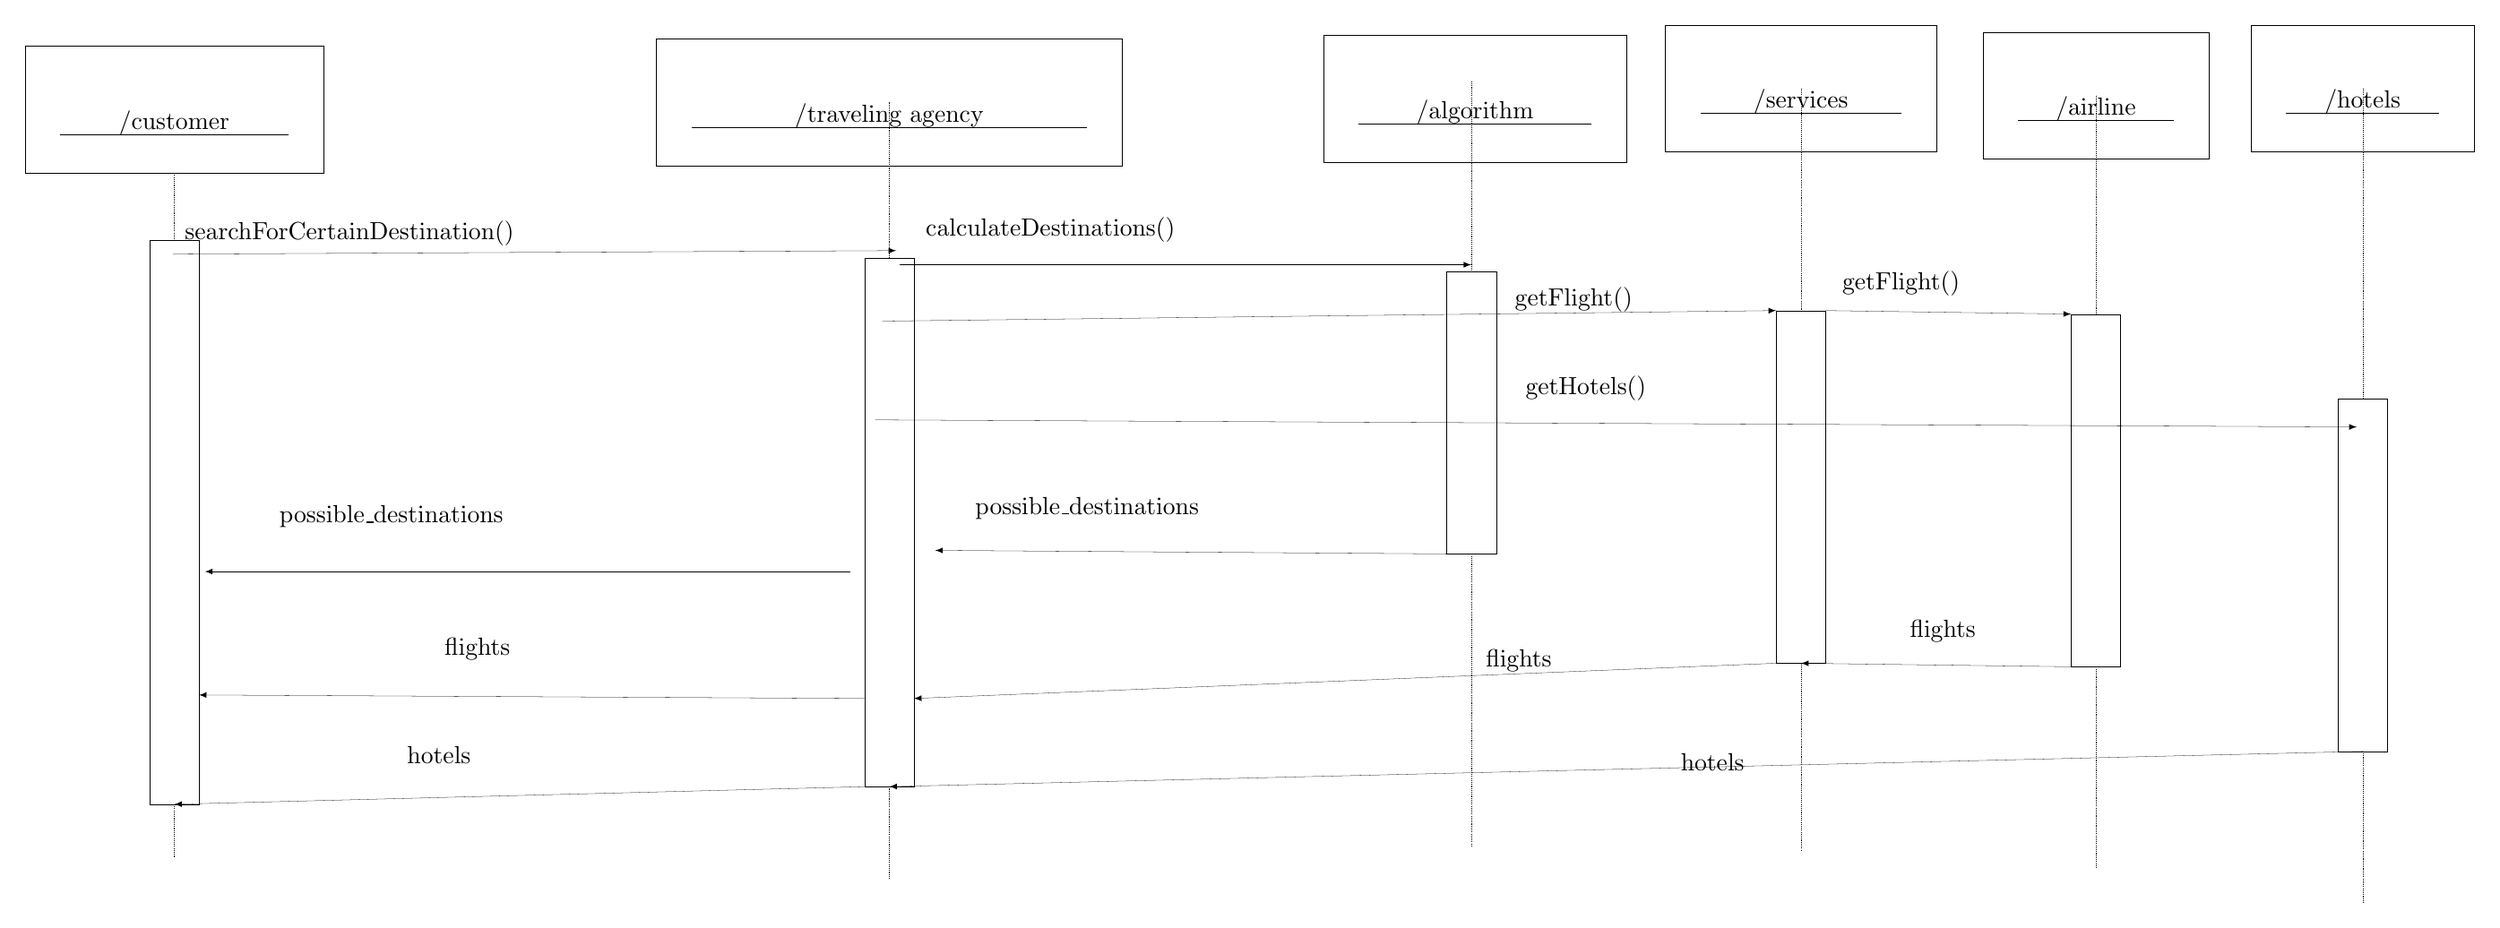
\begin{tikzpicture}
\pgftransformxscale{1.000000}
\pgftransformyscale{-1.000000}
\definecolor{dialinecolor}{rgb}{0.000000, 0.000000, 0.000000}
\pgfsetstrokecolor{dialinecolor}
\definecolor{dialinecolor}{rgb}{1.000000, 1.000000, 1.000000}
\pgfsetfillcolor{dialinecolor}
\pgfsetlinewidth{0.050000\du}
\pgfsetdash{}{0pt}
\pgfsetdash{{0.400000\du}{0.400000\du}}{0\du}
\definecolor{dialinecolor}{rgb}{0.000000, 0.000000, 0.000000}
\pgfsetstrokecolor{dialinecolor}
\draw (2.615000\du,1.550000\du)--(2.615000\du,3.400000\du);
\definecolor{dialinecolor}{rgb}{0.000000, 0.000000, 0.000000}
\pgfsetstrokecolor{dialinecolor}
\draw (2.615000\du,11.400000\du)--(2.615000\du,12.150000\du);
\pgfsetlinewidth{0.100000\du}
\pgfsetdash{}{0pt}
\definecolor{dialinecolor}{rgb}{1.000000, 1.000000, 1.000000}
\pgfsetfillcolor{dialinecolor}
\fill (2.265000\du,3.400000\du)--(2.265000\du,11.400000\du)--(2.965000\du,11.400000\du)--(2.965000\du,3.400000\du)--cycle;
\definecolor{dialinecolor}{rgb}{0.000000, 0.000000, 0.000000}
\pgfsetstrokecolor{dialinecolor}
\draw (2.265000\du,3.400000\du)--(2.265000\du,11.400000\du)--(2.965000\du,11.400000\du)--(2.965000\du,3.400000\du)--cycle;
\pgfsetlinewidth{0.100000\du}
\pgfsetdash{}{0pt}
\definecolor{dialinecolor}{rgb}{1.000000, 1.000000, 1.000000}
\pgfsetfillcolor{dialinecolor}
\fill (0.500000\du,0.650000\du)--(0.500000\du,2.450000\du)--(4.730000\du,2.450000\du)--(4.730000\du,0.650000\du)--cycle;
\definecolor{dialinecolor}{rgb}{0.000000, 0.000000, 0.000000}
\pgfsetstrokecolor{dialinecolor}
\draw (0.500000\du,0.650000\du)--(0.500000\du,2.450000\du)--(4.730000\du,2.450000\du)--(4.730000\du,0.650000\du)--cycle;
% setfont left to latex
\definecolor{dialinecolor}{rgb}{0.000000, 0.000000, 0.000000}
\pgfsetstrokecolor{dialinecolor}
\node at (2.615000\du,1.745000\du){/customer};
% setfont left to latex
\pgfsetlinewidth{0.050000\du}
\definecolor{dialinecolor}{rgb}{0.000000, 0.000000, 0.000000}
\pgfsetstrokecolor{dialinecolor}
\draw (1.000000\du,1.897500\du)--(4.230000\du,1.897500\du);
\pgfsetlinewidth{0.100000\du}
\pgfsetdash{}{0pt}
\definecolor{dialinecolor}{rgb}{1.000000, 1.000000, 1.000000}
\pgfsetfillcolor{dialinecolor}
\fill (9.450000\du,0.550000\du)--(9.450000\du,2.350000\du)--(16.047500\du,2.350000\du)--(16.047500\du,0.550000\du)--cycle;
\definecolor{dialinecolor}{rgb}{0.000000, 0.000000, 0.000000}
\pgfsetstrokecolor{dialinecolor}
\draw (9.450000\du,0.550000\du)--(9.450000\du,2.350000\du)--(16.047500\du,2.350000\du)--(16.047500\du,0.550000\du)--cycle;
% setfont left to latex
\definecolor{dialinecolor}{rgb}{0.000000, 0.000000, 0.000000}
\pgfsetstrokecolor{dialinecolor}
\node at (12.748750\du,1.645000\du){/traveling agency};
% setfont left to latex
\pgfsetlinewidth{0.050000\du}
\definecolor{dialinecolor}{rgb}{0.000000, 0.000000, 0.000000}
\pgfsetstrokecolor{dialinecolor}
\draw (9.950000\du,1.797500\du)--(15.547500\du,1.797500\du);
\pgfsetlinewidth{0.050000\du}
\pgfsetdash{}{0pt}
\pgfsetdash{{0.400000\du}{0.400000\du}}{0\du}
\definecolor{dialinecolor}{rgb}{0.000000, 0.000000, 0.000000}
\pgfsetstrokecolor{dialinecolor}
\draw (12.748750\du,1.450000\du)--(12.748750\du,3.650000\du);
\definecolor{dialinecolor}{rgb}{0.000000, 0.000000, 0.000000}
\pgfsetstrokecolor{dialinecolor}
\draw (12.748750\du,11.150000\du)--(12.748750\du,12.450000\du);
\pgfsetlinewidth{0.100000\du}
\pgfsetdash{}{0pt}
\definecolor{dialinecolor}{rgb}{1.000000, 1.000000, 1.000000}
\pgfsetfillcolor{dialinecolor}
\fill (12.398750\du,3.650000\du)--(12.398750\du,11.150000\du)--(13.098750\du,11.150000\du)--(13.098750\du,3.650000\du)--cycle;
\definecolor{dialinecolor}{rgb}{0.000000, 0.000000, 0.000000}
\pgfsetstrokecolor{dialinecolor}
\draw (12.398750\du,3.650000\du)--(12.398750\du,11.150000\du)--(13.098750\du,11.150000\du)--(13.098750\du,3.650000\du)--cycle;
\pgfsetlinewidth{0.100000\du}
\pgfsetdash{}{0pt}
\definecolor{dialinecolor}{rgb}{1.000000, 1.000000, 1.000000}
\pgfsetfillcolor{dialinecolor}
\fill (18.900000\du,0.500000\du)--(18.900000\du,2.300000\du)--(23.202500\du,2.300000\du)--(23.202500\du,0.500000\du)--cycle;
\definecolor{dialinecolor}{rgb}{0.000000, 0.000000, 0.000000}
\pgfsetstrokecolor{dialinecolor}
\draw (18.900000\du,0.500000\du)--(18.900000\du,2.300000\du)--(23.202500\du,2.300000\du)--(23.202500\du,0.500000\du)--cycle;
% setfont left to latex
\definecolor{dialinecolor}{rgb}{0.000000, 0.000000, 0.000000}
\pgfsetstrokecolor{dialinecolor}
\node at (21.051250\du,1.595000\du){/algorithm};
% setfont left to latex
\pgfsetlinewidth{0.050000\du}
\definecolor{dialinecolor}{rgb}{0.000000, 0.000000, 0.000000}
\pgfsetstrokecolor{dialinecolor}
\draw (19.400000\du,1.747500\du)--(22.702500\du,1.747500\du);
\pgfsetlinewidth{0.050000\du}
\pgfsetdash{}{0pt}
\pgfsetdash{{0.400000\du}{0.400000\du}}{0\du}
\definecolor{dialinecolor}{rgb}{0.000000, 0.000000, 0.000000}
\pgfsetstrokecolor{dialinecolor}
\draw (21.001250\du,1.150000\du)--(21.001250\du,3.850000\du);
\definecolor{dialinecolor}{rgb}{0.000000, 0.000000, 0.000000}
\pgfsetstrokecolor{dialinecolor}
\draw (21.001250\du,7.850000\du)--(21.001250\du,12.000000\du);
\pgfsetlinewidth{0.100000\du}
\pgfsetdash{}{0pt}
\definecolor{dialinecolor}{rgb}{1.000000, 1.000000, 1.000000}
\pgfsetfillcolor{dialinecolor}
\fill (20.651250\du,3.850000\du)--(20.651250\du,7.850000\du)--(21.351250\du,7.850000\du)--(21.351250\du,3.850000\du)--cycle;
\definecolor{dialinecolor}{rgb}{0.000000, 0.000000, 0.000000}
\pgfsetstrokecolor{dialinecolor}
\draw (20.651250\du,3.850000\du)--(20.651250\du,7.850000\du)--(21.351250\du,7.850000\du)--(21.351250\du,3.850000\du)--cycle;
\pgfsetlinewidth{0.100000\du}
\pgfsetdash{}{0pt}
\definecolor{dialinecolor}{rgb}{1.000000, 1.000000, 1.000000}
\pgfsetfillcolor{dialinecolor}
\fill (23.750000\du,0.350000\du)--(23.750000\du,2.150000\du)--(27.592500\du,2.150000\du)--(27.592500\du,0.350000\du)--cycle;
\definecolor{dialinecolor}{rgb}{0.000000, 0.000000, 0.000000}
\pgfsetstrokecolor{dialinecolor}
\draw (23.750000\du,0.350000\du)--(23.750000\du,2.150000\du)--(27.592500\du,2.150000\du)--(27.592500\du,0.350000\du)--cycle;
% setfont left to latex
\definecolor{dialinecolor}{rgb}{0.000000, 0.000000, 0.000000}
\pgfsetstrokecolor{dialinecolor}
\node at (25.671250\du,1.445000\du){/services};
% setfont left to latex
\pgfsetlinewidth{0.050000\du}
\definecolor{dialinecolor}{rgb}{0.000000, 0.000000, 0.000000}
\pgfsetstrokecolor{dialinecolor}
\draw (24.250000\du,1.597500\du)--(27.092500\du,1.597500\du);
\pgfsetlinewidth{0.050000\du}
\pgfsetdash{}{0pt}
\pgfsetdash{{0.400000\du}{0.400000\du}}{0\du}
\definecolor{dialinecolor}{rgb}{0.000000, 0.000000, 0.000000}
\pgfsetstrokecolor{dialinecolor}
\draw (25.671250\du,1.250000\du)--(25.671250\du,4.400000\du);
\definecolor{dialinecolor}{rgb}{0.000000, 0.000000, 0.000000}
\pgfsetstrokecolor{dialinecolor}
\draw (25.671250\du,9.400000\du)--(25.671250\du,12.050000\du);
\pgfsetlinewidth{0.100000\du}
\pgfsetdash{}{0pt}
\definecolor{dialinecolor}{rgb}{1.000000, 1.000000, 1.000000}
\pgfsetfillcolor{dialinecolor}
\fill (25.321250\du,4.400000\du)--(25.321250\du,9.400000\du)--(26.021250\du,9.400000\du)--(26.021250\du,4.400000\du)--cycle;
\definecolor{dialinecolor}{rgb}{0.000000, 0.000000, 0.000000}
\pgfsetstrokecolor{dialinecolor}
\draw (25.321250\du,4.400000\du)--(25.321250\du,9.400000\du)--(26.021250\du,9.400000\du)--(26.021250\du,4.400000\du)--cycle;
\pgfsetlinewidth{0.100000\du}
\pgfsetdash{}{0pt}
\definecolor{dialinecolor}{rgb}{1.000000, 1.000000, 1.000000}
\pgfsetfillcolor{dialinecolor}
\fill (28.250000\du,0.450000\du)--(28.250000\du,2.250000\du)--(31.452500\du,2.250000\du)--(31.452500\du,0.450000\du)--cycle;
\definecolor{dialinecolor}{rgb}{0.000000, 0.000000, 0.000000}
\pgfsetstrokecolor{dialinecolor}
\draw (28.250000\du,0.450000\du)--(28.250000\du,2.250000\du)--(31.452500\du,2.250000\du)--(31.452500\du,0.450000\du)--cycle;
% setfont left to latex
\definecolor{dialinecolor}{rgb}{0.000000, 0.000000, 0.000000}
\pgfsetstrokecolor{dialinecolor}
\node at (29.851250\du,1.545000\du){/airline};
% setfont left to latex
\pgfsetlinewidth{0.050000\du}
\definecolor{dialinecolor}{rgb}{0.000000, 0.000000, 0.000000}
\pgfsetstrokecolor{dialinecolor}
\draw (28.750000\du,1.697500\du)--(30.952500\du,1.697500\du);
\pgfsetlinewidth{0.050000\du}
\pgfsetdash{}{0pt}
\pgfsetdash{{0.400000\du}{0.400000\du}}{0\du}
\definecolor{dialinecolor}{rgb}{0.000000, 0.000000, 0.000000}
\pgfsetstrokecolor{dialinecolor}
\draw (29.851250\du,1.350000\du)--(29.851250\du,4.450000\du);
\definecolor{dialinecolor}{rgb}{0.000000, 0.000000, 0.000000}
\pgfsetstrokecolor{dialinecolor}
\draw (29.851250\du,9.450000\du)--(29.851250\du,12.300000\du);
\pgfsetlinewidth{0.100000\du}
\pgfsetdash{}{0pt}
\definecolor{dialinecolor}{rgb}{1.000000, 1.000000, 1.000000}
\pgfsetfillcolor{dialinecolor}
\fill (29.501250\du,4.450000\du)--(29.501250\du,9.450000\du)--(30.201250\du,9.450000\du)--(30.201250\du,4.450000\du)--cycle;
\definecolor{dialinecolor}{rgb}{0.000000, 0.000000, 0.000000}
\pgfsetstrokecolor{dialinecolor}
\draw (29.501250\du,4.450000\du)--(29.501250\du,9.450000\du)--(30.201250\du,9.450000\du)--(30.201250\du,4.450000\du)--cycle;
\pgfsetlinewidth{0.100000\du}
\pgfsetdash{}{0pt}
\pgfsetdash{}{0pt}
\pgfsetbuttcap
{
\definecolor{dialinecolor}{rgb}{0.000000, 0.000000, 0.000000}
\pgfsetfillcolor{dialinecolor}
% was here!!!
\pgfsetarrowsend{latex}
\definecolor{dialinecolor}{rgb}{0.000000, 0.000000, 0.000000}
\pgfsetstrokecolor{dialinecolor}
\draw (2.600000\du,3.600000\du)--(12.850000\du,3.550000\du);
}
% setfont left to latex
\definecolor{dialinecolor}{rgb}{0.000000, 0.000000, 0.000000}
\pgfsetstrokecolor{dialinecolor}
\node[anchor=west] at (7.600000\du,6.400000\du){};
% setfont left to latex
\definecolor{dialinecolor}{rgb}{0.000000, 0.000000, 0.000000}
\pgfsetstrokecolor{dialinecolor}
\node[anchor=west] at (4.500000\du,2.950000\du){};
% setfont left to latex
\definecolor{dialinecolor}{rgb}{0.000000, 0.000000, 0.000000}
\pgfsetstrokecolor{dialinecolor}
\node[anchor=west] at (2.650000\du,3.300000\du){searchForCertainDestination()};
\pgfsetlinewidth{0.100000\du}
\pgfsetdash{}{0pt}
\pgfsetdash{}{0pt}
\pgfsetbuttcap
{
\definecolor{dialinecolor}{rgb}{0.000000, 0.000000, 0.000000}
\pgfsetfillcolor{dialinecolor}
% was here!!!
\pgfsetarrowsend{latex}
\definecolor{dialinecolor}{rgb}{0.000000, 0.000000, 0.000000}
\pgfsetstrokecolor{dialinecolor}
\draw (12.900000\du,3.750000\du)--(21.000000\du,3.750000\du);
}
% setfont left to latex
\definecolor{dialinecolor}{rgb}{0.000000, 0.000000, 0.000000}
\pgfsetstrokecolor{dialinecolor}
\node[anchor=west] at (13.150000\du,3.250000\du){calculateDestinations()};
\pgfsetlinewidth{0.100000\du}
\pgfsetdash{}{0pt}
\pgfsetdash{}{0pt}
\pgfsetbuttcap
{
\definecolor{dialinecolor}{rgb}{0.000000, 0.000000, 0.000000}
\pgfsetfillcolor{dialinecolor}
% was here!!!
\pgfsetarrowsend{latex}
\definecolor{dialinecolor}{rgb}{0.000000, 0.000000, 0.000000}
\pgfsetstrokecolor{dialinecolor}
\draw (12.650000\du,4.550000\du)--(25.321250\du,4.400000\du);
}
% setfont left to latex
\definecolor{dialinecolor}{rgb}{0.000000, 0.000000, 0.000000}
\pgfsetstrokecolor{dialinecolor}
\node[anchor=west] at (21.500000\du,4.250000\du){getFlight()};
\pgfsetlinewidth{0.100000\du}
\pgfsetdash{}{0pt}
\pgfsetdash{}{0pt}
\pgfsetbuttcap
{
\definecolor{dialinecolor}{rgb}{0.000000, 0.000000, 0.000000}
\pgfsetfillcolor{dialinecolor}
% was here!!!
\pgfsetarrowsend{latex}
\definecolor{dialinecolor}{rgb}{0.000000, 0.000000, 0.000000}
\pgfsetstrokecolor{dialinecolor}
\draw (26.021250\du,4.400000\du)--(29.501250\du,4.450000\du);
}
% setfont left to latex
\definecolor{dialinecolor}{rgb}{0.000000, 0.000000, 0.000000}
\pgfsetstrokecolor{dialinecolor}
\node[anchor=west] at (26.140000\du,4.020000\du){getFlight()};
\pgfsetlinewidth{0.100000\du}
\pgfsetdash{}{0pt}
\pgfsetdash{}{0pt}
\pgfsetbuttcap
{
\definecolor{dialinecolor}{rgb}{0.000000, 0.000000, 0.000000}
\pgfsetfillcolor{dialinecolor}
% was here!!!
\pgfsetarrowsend{latex}
\definecolor{dialinecolor}{rgb}{0.000000, 0.000000, 0.000000}
\pgfsetstrokecolor{dialinecolor}
\draw (29.501250\du,9.450000\du)--(25.671250\du,9.400000\du);
}
\pgfsetlinewidth{0.100000\du}
\pgfsetdash{}{0pt}
\pgfsetdash{}{0pt}
\pgfsetbuttcap
{
\definecolor{dialinecolor}{rgb}{0.000000, 0.000000, 0.000000}
\pgfsetfillcolor{dialinecolor}
% was here!!!
\pgfsetarrowsend{latex}
\definecolor{dialinecolor}{rgb}{0.000000, 0.000000, 0.000000}
\pgfsetstrokecolor{dialinecolor}
\draw (20.651250\du,7.850000\du)--(13.400000\du,7.800000\du);
}
\pgfsetlinewidth{0.100000\du}
\pgfsetdash{}{0pt}
\pgfsetdash{}{0pt}
\pgfsetbuttcap
{
\definecolor{dialinecolor}{rgb}{0.000000, 0.000000, 0.000000}
\pgfsetfillcolor{dialinecolor}
% was here!!!
\pgfsetarrowsend{latex}
\definecolor{dialinecolor}{rgb}{0.000000, 0.000000, 0.000000}
\pgfsetstrokecolor{dialinecolor}
\draw (12.200000\du,8.100000\du)--(3.050000\du,8.100000\du);
}
% setfont left to latex
\definecolor{dialinecolor}{rgb}{0.000000, 0.000000, 0.000000}
\pgfsetstrokecolor{dialinecolor}
\node[anchor=west] at (13.850000\du,7.200000\du){possible\_destinations};
% setfont left to latex
\definecolor{dialinecolor}{rgb}{0.000000, 0.000000, 0.000000}
\pgfsetstrokecolor{dialinecolor}
\node[anchor=west] at (3.990000\du,7.320000\du){possible\_destinations};
% setfont left to latex
\definecolor{dialinecolor}{rgb}{0.000000, 0.000000, 0.000000}
\pgfsetstrokecolor{dialinecolor}
\node[anchor=west] at (27.100000\du,8.950000\du){flights};
\pgfsetlinewidth{0.100000\du}
\pgfsetdash{}{0pt}
\pgfsetdash{}{0pt}
\pgfsetbuttcap
{
\definecolor{dialinecolor}{rgb}{0.000000, 0.000000, 0.000000}
\pgfsetfillcolor{dialinecolor}
% was here!!!
\pgfsetarrowsend{latex}
\definecolor{dialinecolor}{rgb}{0.000000, 0.000000, 0.000000}
\pgfsetstrokecolor{dialinecolor}
\draw (25.321250\du,9.400000\du)--(13.098750\du,9.900000\du);
}
\pgfsetlinewidth{0.100000\du}
\pgfsetdash{}{0pt}
\pgfsetdash{}{0pt}
\pgfsetbuttcap
{
\definecolor{dialinecolor}{rgb}{0.000000, 0.000000, 0.000000}
\pgfsetfillcolor{dialinecolor}
% was here!!!
\pgfsetarrowsend{latex}
\definecolor{dialinecolor}{rgb}{0.000000, 0.000000, 0.000000}
\pgfsetstrokecolor{dialinecolor}
\draw (12.398750\du,9.900000\du)--(2.965000\du,9.850000\du);
}
% setfont left to latex
\definecolor{dialinecolor}{rgb}{0.000000, 0.000000, 0.000000}
\pgfsetstrokecolor{dialinecolor}
\node[anchor=west] at (21.090000\du,9.370000\du){flights};
% setfont left to latex
\definecolor{dialinecolor}{rgb}{0.000000, 0.000000, 0.000000}
\pgfsetstrokecolor{dialinecolor}
\node[anchor=west] at (6.330000\du,9.195000\du){flights};
\pgfsetlinewidth{0.100000\du}
\pgfsetdash{}{0pt}
\definecolor{dialinecolor}{rgb}{1.000000, 1.000000, 1.000000}
\pgfsetfillcolor{dialinecolor}
\fill (32.050000\du,0.350000\du)--(32.050000\du,2.150000\du)--(35.217500\du,2.150000\du)--(35.217500\du,0.350000\du)--cycle;
\definecolor{dialinecolor}{rgb}{0.000000, 0.000000, 0.000000}
\pgfsetstrokecolor{dialinecolor}
\draw (32.050000\du,0.350000\du)--(32.050000\du,2.150000\du)--(35.217500\du,2.150000\du)--(35.217500\du,0.350000\du)--cycle;
% setfont left to latex
\definecolor{dialinecolor}{rgb}{0.000000, 0.000000, 0.000000}
\pgfsetstrokecolor{dialinecolor}
\node at (33.633750\du,1.445000\du){/hotels};
% setfont left to latex
\pgfsetlinewidth{0.050000\du}
\definecolor{dialinecolor}{rgb}{0.000000, 0.000000, 0.000000}
\pgfsetstrokecolor{dialinecolor}
\draw (32.550000\du,1.597500\du)--(34.717500\du,1.597500\du);
\pgfsetlinewidth{0.050000\du}
\pgfsetdash{}{0pt}
\pgfsetdash{{0.400000\du}{0.400000\du}}{0\du}
\definecolor{dialinecolor}{rgb}{0.000000, 0.000000, 0.000000}
\pgfsetstrokecolor{dialinecolor}
\draw (33.633750\du,1.250000\du)--(33.633750\du,5.650000\du);
\definecolor{dialinecolor}{rgb}{0.000000, 0.000000, 0.000000}
\pgfsetstrokecolor{dialinecolor}
\draw (33.633750\du,10.650000\du)--(33.633750\du,12.800000\du);
\pgfsetlinewidth{0.100000\du}
\pgfsetdash{}{0pt}
\definecolor{dialinecolor}{rgb}{1.000000, 1.000000, 1.000000}
\pgfsetfillcolor{dialinecolor}
\fill (33.283750\du,5.650000\du)--(33.283750\du,10.650000\du)--(33.983750\du,10.650000\du)--(33.983750\du,5.650000\du)--cycle;
\definecolor{dialinecolor}{rgb}{0.000000, 0.000000, 0.000000}
\pgfsetstrokecolor{dialinecolor}
\draw (33.283750\du,5.650000\du)--(33.283750\du,10.650000\du)--(33.983750\du,10.650000\du)--(33.983750\du,5.650000\du)--cycle;
\pgfsetlinewidth{0.100000\du}
\pgfsetdash{}{0pt}
\pgfsetdash{}{0pt}
\pgfsetbuttcap
{
\definecolor{dialinecolor}{rgb}{0.000000, 0.000000, 0.000000}
\pgfsetfillcolor{dialinecolor}
% was here!!!
\pgfsetarrowsend{latex}
\definecolor{dialinecolor}{rgb}{0.000000, 0.000000, 0.000000}
\pgfsetstrokecolor{dialinecolor}
\draw (12.550000\du,5.950000\du)--(33.550000\du,6.050000\du);
}
% setfont left to latex
\definecolor{dialinecolor}{rgb}{0.000000, 0.000000, 0.000000}
\pgfsetstrokecolor{dialinecolor}
\node[anchor=west] at (21.650000\du,5.500000\du){getHotels()};
\pgfsetlinewidth{0.100000\du}
\pgfsetdash{}{0pt}
\pgfsetdash{}{0pt}
\pgfsetbuttcap
{
\definecolor{dialinecolor}{rgb}{0.000000, 0.000000, 0.000000}
\pgfsetfillcolor{dialinecolor}
% was here!!!
\pgfsetarrowsend{latex}
\definecolor{dialinecolor}{rgb}{0.000000, 0.000000, 0.000000}
\pgfsetstrokecolor{dialinecolor}
\draw (33.633750\du,10.650000\du)--(12.748750\du,11.150000\du);
}
% setfont left to latex
\definecolor{dialinecolor}{rgb}{0.000000, 0.000000, 0.000000}
\pgfsetstrokecolor{dialinecolor}
\node[anchor=west] at (23.850000\du,10.800000\du){hotels};
\pgfsetlinewidth{0.100000\du}
\pgfsetdash{}{0pt}
\pgfsetdash{}{0pt}
\pgfsetbuttcap
{
\definecolor{dialinecolor}{rgb}{0.000000, 0.000000, 0.000000}
\pgfsetfillcolor{dialinecolor}
% was here!!!
\pgfsetarrowsend{latex}
\definecolor{dialinecolor}{rgb}{0.000000, 0.000000, 0.000000}
\pgfsetstrokecolor{dialinecolor}
\draw (12.398750\du,11.150000\du)--(2.615000\du,11.400000\du);
}
% setfont left to latex
\definecolor{dialinecolor}{rgb}{0.000000, 0.000000, 0.000000}
\pgfsetstrokecolor{dialinecolor}
\node[anchor=west] at (5.800000\du,10.700000\du){hotels};
\end{tikzpicture}
%
\endgroup

\centerline{\includegraphics[scale=0.4]{Diagram1}}
GeneralizableElements:classes,Association, Stereotypes, Signals and Use Cases
\subsection{Requirements elicitation}
gathering requirements from end-users,customers and other stakeholders
\subsection{stakeholder(user-centered design)}
Definition. A stakeholder in the architecture of a system is an individual, team, organization, or classes thereof, having an interest in the realization of the system. 
\newline
Primary stakeholder: people who i saffected of the putcome of the project(users)\newline
secondary:people who can affect the outcome of the project but is not themself affected of it(designers)
 \newline
 Direct stakeholder: Concerned with the day to day activities of the project(designers)
 \newline
 Indirect stakeholder: people affected by the end result(users)
 \subsection{natural language in requirements}
 pros:
 \newline
 almost everyone can understand them\\
 elmost anyone can write them
 cons:
 \newline
 the interpretation can vary depending on reader
 \\one requirement can be written in so many ways
 \\There is no easy way to modularise natural language requirements
 
 %DESIGN AND ARCHITECTURE
\section{Design \& Architecture}
\subsection{architectural view}
\begin{itemize}
\item Logical view : The logical view is concerned with the functionality that the system provides to end-users. 
\item Development view : The development view illustrates a system from a programmer's perspective
\item Process view : The process view deals with the dynamic aspects of the system, explains the system processes and how they communicate
\item Physical view : The physical view depicts the system from a system engineer's point of view.
\end{itemize}
\subsection{obserber pattern}
 is a software design pattern in which an object, called the subject, maintains a list of its dependents, called observers, and notifies them automatically of any state changes, 
 \subsection{client-server}
 two-tier,thin-client:-heavy load on server,-significant network traffic\\
 two-tier.fat client:+distribute workload on clients,-needs to update software on server//
 three-tier:+map each layer on separate hardware,+possibility for load-balancing
\subsection{layered architecture}
pros:
\begin{itemize}
\item reduced complexity
\item easier to maintain code
\item easier to add new functionality
\item easier to test
\item allows to reuse code
\end{itemize}
cons:
\begin{itemize}
\item restricting communication to adjacent layers
\item keeping coupling between layers reduced.
\end{itemize}
\subsection{Facade pattern}
hide complexity of a system from the user
\subsection{implementation view}
Software packages, libraries, frameworks, classes,
 \subsection{cohesion and coupling}
 Cohesion:How uniform and easy understanding the code in software is. High cohesion is prefered
 \\Coupling: how much all the modules are entagled into another. Low coupling is prefered
 \subsection{pipe-and-filters}
 advantages:
 \\simplicity-Allows designer to understand overall input/output behavior of a system in terms of individual filters
 \\Maintenance and reuse
 \\Concurrent Execution –Each filter can be implemented as a separate task and be executed in parallel with other filters.\\
 disadvantages:
 Interactive transformations are difficult – Filters being independent entities designer has to think of each filter as providing a complete transformation of input data to output data.
 \\No filter cooperation.
 \\Performance – may force a lowest common denominator on data transmission
 \subsection{strategy pattern}
 In computer programming, the strategy pattern (also known as the policy pattern) is a software design pattern that enables an algorithm's behavior to be selected at runtime. The strategy pattern:
 \\
defines a family of algorithms\\
encapsulates each algorithm\\
makes the algorithms interchangeable within that family.\\
\centerline{\includegraphics[scale=0.6]{Strategy}}
\subsection{Behavioral design patterns}
This design patterns is all about Class's objects communication. Behavioral patterns are those patterns that are most specifically concerned with communication between objects.

%TESTING
\section{Testing}
A fault(bug) leads to an error that can lead to a failure of the system
\subsection{function testing}
bases its test cases on the specifications of the software component under test
\subsection{performance test}
is generally executed to determine how a system or sub-system performs in terms of responsiveness and stability under a particular workload
\subsection{acceptance testing}
 is a test conducted to determine if the requirements of a specification or contract are met. 
 \subsection{installation testing}
 An installation test assures that the system is installed correctly and working at actual customer's hardware.
\subsection{continuous integration}
Everytime a developer commit a piece of code a build server builds the project and runs some tests to see that the integration with the new code works.
\subsection{configuration management}
Lock-modify-unlock: When you check something out you lock that object so it cant be modified.
\\Centralized-modify-merge: When a conflict occur the system tries to merge the changes. If its not able to you can merge the chages manually.
\\Decentralized-modify-merge: The merging is done off the system. You ahve to mail patches around and then one person manually patches it and commits it. 
\subsection{test case}
every test-case needs test-case ID,inputs,expected outputs
\subsection{daily build}
Each day the software is built to make shure the program can compile and tests can be run to make shure no new bugs has appeared during the day. This can be automated and the tests can be some smoke test or it can be done manually by a person.
\subsection{smoke test}
Very basic fast tests. For example does the program run?, does it open a windows?, does the main button do anything. 
\subsection{code-coverage(white box testing)}
Code-coverage means how much of the code in the project is being tested. For example a project with 100\% code-coverage means that every single line of code have been tested. 
\subsection{big-bang-testing}
A system wide test that test all modules at once. Very time efficiant
\subsection{top-down}
The modules are split up into levels and are tested one level at a time starting from the upper level. For the lower level functions stubs are written. For complex systems with alot of levels alot of stubs might have to be written.provides an early outline of the overall program helping to finddesign errors early on
\subsection{bottom-up}
The program is split up into levels and the lower ones are tested first. To drive them you write drivers to send them test-casesdrivers are easi
er to
produce than stubs and because the tester is workin
g upwards
from the bottom layer, they have a more thorough
understanding of the functioning of the lower layer
modules
and thus have a far better idea of how to create su
itable tests
for the upper layer modules
\subsection{sandwhich testing}
It is a combination of both Top-down and Bottom-up
integration testing. A target layer is defined in the middle of the pro
gram and testing is carried out
from the top and bottom layers to converge at this
target layer.
•It has the advantages that the top and bottom laye
rs can be tested in parallel and
can lower the need for stubs and drivers. However, it can be more complex to plan and select
ing the ‘best’ target layer can
be difficult. 

%PLANNING AND PROCESS
\section{Planning \& Processes}
\subsection{project plan}
project description:
\begin{itemize}
\item Background to the project
\item Relevant constraints (budget etc.)
\item Project Goal
\item Start and expected end date
\end{itemize}
project organization
\begin{itemize}
\item Roles
\item Knowledge / skill
\item Training
\item Communication and reports
\end{itemize}
Time and Resource Plan
\begin{itemize}
\item Milestones
\item Tollgates
\item Deliverables
\item Activities
\item Resources
\end{itemize}
Risk Management
\begin{itemize}
\item Risks,Probability and Impact
\item Mitigation and Contingency plan
\end{itemize}

\subsection{scrum}
\begin{itemize}
\item burn down chart:is a graphical representation of work left to do versus time. The outstanding work (or backlog) is often on the vertical axis, with time along the horizontal.
\item daily scrum meeting:
    What have you done since yesterday?
    What are you planning to do today?
    Any impediments/stumbling blocks? Problems are the scrum master responability to resolve

\end{itemize}
\subsection{gantt chart}
\begin{itemize}
\item task: for example "fix bug nr 34"
\item phase: for example "design phase"
\item milestone: for example "network module finished"
\item tollgate: for example "design stop"
\end{itemize}
\subsection{extreme programming(agile)}
practises:
\begin{itemize}
\item Pair programming: means that all code is produced by two people programming on one task on one workstation
\item User stories (planning): desribes features
\item Small releases (building blocks): With XP, you develop and deliver the application in a series of small, frequently updated versions.
\item Collective ownership: No one person owns or is responsible for individual code segments.
\item Coding standard: All team members write code in the same way, using the same styles and formats.
\end{itemize}
\subsection{four parameters}
calender time,resources,features,quality
\subsection{waterfall model}
good with fix-rpice contracts
pros:
\begin{itemize}
\item This model is simple and easy to understand and use.
\item It is easy to manage due to the rigidity of the model 
\item Waterfall model works well for smaller projects where requirements are very well understood.
\end{itemize}
cons:
\begin{itemize}
\item Once an application is in the testing stage, it is very difficult to go back and change something that was not well-thought out in the concept stage.
\item No working software is produced until late during the life cycle.
\item Not suitable for the projects where requirements are at a moderate to high risk of changing.
\end{itemize}
\subsection{Agile methods}
egile manifesto:
\begin{itemize}
\item Individuals and interactions: in agile development, self-organization and motivation are important, as are interactions like co-location and pair programming.
\item Working software: working software will be more useful and welcome than just presenting documents to clients in meetings.
\item Customer collaboration: requirements cannot be fully collected at the beginning of the software development cycle, therefore continuous customer or stakeholder involvement is very important.
\item Responding to change: agile development is focused on quick responses to change and continuous development.

\end{itemize}
\begin{itemize}
\item adaptive planning
\item evolutionary development
\item early delivery
\item continuous improvement
\item encourages rapid and flexible response to change
\end{itemize}
pros:
\begin{itemize}
\item Customer satisfaction by rapid, continuous delivery of useful software
\item People and interactions are emphasized rather than process and tools.
\item Customers, developers and testers constantly interact with each other.
\item Working software is delivered frequently (weeks rather than months).
\item Face-to-face conversation is the best form of communication.
\item Close, daily cooperation between business people and developers.
\item Continuous attention to technical excellence and good design.
\item Regular adaptation to changing circumstances.
\item Even late changes in requirements are welcomed
\end{itemize}
cons:
\begin{itemize}
\item In case of some software deliverables, especially the large ones, it is difficult to assess the effort required at the beginning of the software development life cycle.

\item There is lack of emphasis on necessary designing and documentation.
\item The project can easily get taken off track if the customer representative is not clear what final outcome that they want.
\item Only senior programmers are capable of taking the kind of decisions required during the development process. Hence it has no place for newbie programmers, unless combined with experienced resources.
\end{itemize}
when:
\begin{itemize}
\item when change is needed during the project
\item when a project needs to start right away
\item major decisions can be made during the development
\end{itemize}
when not:
\begin{itemize}
\item the development team is spread over the world. You need face to face communication
\item if you dont have a project manager on site that can make quick decisions
\item if people affected by the project need complete clarity on solutions before starting the project
\item You have a fix deadline with a fixed set of requirements
\end{itemize}
\subsection{iterative model}
no overhead
\\pros
\begin{itemize}
\item building and improving the product step by step. Hence we can track the defects at early stages
\item we can get the reliable user feedback.
\item ess time is spent on documenting and more time is given for designing
\end{itemize}
cons:
\begin{itemize}
\item Each phase of an iteration is rigid with no overlaps
\item Costly system architecture or design issues may arise because not all requirements are gathered up front for the entire lifecycle
\end{itemize}
\subsection{incremental model}
The projects consists of alot of small builds which become greater with time with more features added each time. \\
pros:\\
generate working software quickly
\\easier to test and debug with small iterations
\\customers can respond to each built
\\cons:
\\requires good planning and design
\\needs a clear and complete definition of the whole system so it can be broken down
\\resulting cost might be greater
\\addiotional functionality that is added might arise problems related to the system design 
\subsection{risk planning}
for example:
$$identify\: risk\rightarrow analyze\rightarrow plan\rightarrow monitor \rightarrow (respond)$$
Risk avoidance:
\\ for example not taking on a project and thuse avoiding the risk that comes with it.
\\risk transfer:
for example using a subcontractor for some part of the project that your company do not have the knowledge of.
\\risk acceptance:
you accept that there are a risk and you put it on a watch list and take no further action.
\\risk mitigation:
planning and taking actions to reduce the effects of the risks. For example don't start any war that might end in a terrorist attack.
\\Contingency plan: minimize the effects if the worst would happen. Don't let alot of the employes travel on the same plan because there might be a terrorist attack.

\subsection{prototype model}
Remainds alot of incremental model. You build a prototype of the system to find out what is missing and what needs to be refind or added to it and you refine the prototype. Itś good for system with alot of end-user interaction such as online systems and web interfaces. 
\\pros:
\\users are involved in the development
\\errors can be detected early
\\missing functionality can be identified easily
\\cons:
\\leads to implementation then repairing
\\may increase complexity of system

%QUALITY FACTORS
\section{Quality factors}
\subsection{usability testing}
users test the software and give feedback
\subsection{usability inspection}
experts test the software without end-users
\subsection{depth in the inheritance tree}
greater depth means greater complexity
\subsection{cylomatic complexity}
It directly measures the number of linearly independent paths through a program's source code.
\subsection{software inspection}
peer review by trained individuals who look for defects using a well defined process.The goal of the inspection is to identify defects
\\roles
\begin{itemize}
\item Author: The person who created the work product being inspected.
\item Moderator: This is the leader of the inspection. The moderator plans the inspection and coordinates it.
\item Reader: The person reading through the documents, one item at a time. The other inspectors then point out defects.
\item Recorder/Scribe: The person that documents the defects that are found during the inspection.
\item Inspector: The person that examines the work product to identify possible defects.

\end{itemize}
\subsection{software audit}
is a type of software review in which one or more auditors who are not members of the software development organization conduct "An independent examination of a software product, software process, or set of software processes to assess compliance with specifications, standards, contractual agreements, or other criteria"
\subsection{maintainability}
How easy the software is to maintain meaning does the code follow any standars, are everything well documented an so on.
\subsection{performance}
How fast the software respons and how efficiently it uses ram and harddrive space. For example a software that makes some easy calculations cannot use 16gb of ram.
\subsection{scalability}
Can run on newer machines(vertical scaling). Can run on several machines/multi proccesing (horizontal scaling).
\subsection{flexability}
possible to add/remove modules without breaking the system. 
\subsection{reliability}
Software reliability is the probability of the software components of producing incorrect output. Software should not wear out and continue to operate after a bad result.
\subsection{availability}
Ao = (total time - down time) / total time.
More os less how available the system is. A system with high availability seldom crashes and when it crashes id recovers fast.
\subsection{usability}
How easy the system is to use. Mostly through UI:s
\subsection{portability}
Can it run on several platforms?
\subsection{correctness and functionality}
Does the software have all the functionality stated in the specification?
\subsection{cmmi}
maturity level:
here are five maturity levels. Maturity level ratings are awarded for levels 2 through 5.
\\process areas:
indicating the aspects of product and service development that are to be covered by organizational processes. 
nivå 1\\
Företaget har ingen standardiserad process (arbetssätt) för utveckling av mjukvara. Det saknas också projektuppföljning, som skulle kunna hjälpa till att göra säkrare skattningar av kostnader och löptider för framtida projekt. Målet för detta steg är att få grundläggande kontroll över tidsplaner och kostnader.
\\nivå 2
\\Företaget har installerat processer för konfigurationshantering, men för övrigt brukar alla projekt drivas enligt projektledarens eget tycke, med viss koordination. Grundläggande statistisk uppföljning görs av åtaganden, kostnader, tidsplaner och förändringar.
\end{document}